\chapter{Návrh riešenia}
Na to aby sme boli schopní merať a porovnávať pamäťovú hĺbku sietí, museli sme si
zvoliť vhodné trénovacie dáta, zadefinovať si spôsob merania pamäťovej hĺbky,
sietí a tiež spôsob vyhodnocovania výsledkov.

\section{Pamäťová hĺbka neurónovej siete}
Hĺbka pamäti vyjadruje dĺžku historického kontextu, ktorý má ešte vplyv na aktuálny výstup siete.
Ak je hĺbka pamäti $N$, vstupy v čase menšom ako $(T - N)$ nemajú vplyv na výstup siete v čase $T$.

\section{Určovanie hĺbky pamäte rekurentnej SOM}
Hĺbku pamäte pre konkrétny neurón v sieti určíme ako dĺžku najdlhšej spoločnej postfixovej
podpostupností znakov v množine historii posuvných okien neurónu, pre ktoré bol neurón víťazom.
Dĺžku najdlhšej podpostupnosti budeme určovať od konca sekvencií v množine.
Pamäťovú hĺbku celej siete následne určíme ako vážený priemer nameraných pamäťových hĺbok jednotlivých neurónov, 
kde váha pamäťovej hĺbky neurónu bude určená počtom podpostupností uložených v pamäťovom okne neurónu.
(teda koľko krát bol neurón víťazom počas trénovania).
Neuróny, ktoré neboli víťazom pre žiadny vstup (majú prázdne pamäťové okno)
sa do celkovej pamäťovej hĺbky nezapočítavajú, čiže nemajú žiadny vplyv na pamäťovú hĺbku siete.
Neuróny, ktoré boli víťazom iba pre jeden vstup, majú pamäťovú hĺbku rovnú dĺžke uloženej sekvencie, čiže dĺžke pamäťového okna na trénovacej množine.
Vo výslednej pamäťovej hĺbke majú mať však takéto neuróny, ktoré boli víťazom iba pre jeden vstup, nízku váhu oproti ostatným neurónom.
Preto priemer pamäťových hĺbok jednotlivých neurónov musí byť vážený, aby neuróny, 
ktoré boli víťazmi pre väčší počet vstupov mali vyššiu váhu vo výslednej pamäťovej hĺbke siete, ako neuróny, ktoré boli víťazmi pre menší počet vstupov.
Po každej trénovacej epoche (prechode trénovacou množinou) budeme vedieť určiť veľkosť pamäťovej hĺbky mapy.

Vďaka tomu, že neuróny rekurentných sietí majú okrem normálnych váh aj kontextové váhy a samotný kontext, 
ktoré uchovávajú informácie z predchádzajúcich krokov, môže sa stať, že rovnaké písmeno zo vstupnej sekvencie 
bude mať rôzne víťazné neuróny počas trénovania. Táto vlastnosť rekurentných SOM spôsobuje to, že majú pamäťovú hĺbku, ktorú dokážeme merať.

Samotná pamäťová hĺbka je relatívna a závisí aj od veľkosti posuvného okna (sliding window) na trénovacej množine.
Veľkosť posuvného okna musí byť dostatočne veľká, väčšia ako maximálna nájdená
dĺžka spoločnej postfixovej podpostupnosti pre nejaký neurón, ale zároveň nie príliš veľká, aby sme zbytočne neskresľovali výsledky neurónmi, ktoré boli víťazmi iba pre jeden vstup.
Hľadanie optimálnej veľkosti posuvného okna je súčasťou nášho experimentu.

\section{Metóda uchovávania informácii v SOM}
Na to aby sme boli schopní odmerať pamäťovú hĺbku SOM, potrebujeme si pamätať v jednotlivých
neurónoch informáciu o tom, pre ktoré vstupy bol daný neurón víťazom.
Každý neurón bude mať množinu vstupov, v ktorej si pamätá pre aký vstup bol počas trénovania víťazom. 
Nestačí však ukladať iba samotný vstup, pretože by sme prišli o historický kontext pre daný vstup, 
ktorý je nevyhnutný pri určovaní pamäťovej hĺbky. 
Preto si neukladáme iba aktuálny vstup (aktuálne písmeno), 
ale $k$ posledných písmen z trénovacej sekvencie.
Toto sa nazýva posuvné okno (ang. sliding window) na vstupnej množine. 
Všetky takéto množiny spolu tvoria dokopy tzv. receptívne pole SOM.
Po natrénovaní siete viem z týchto okien vytvoriť hitmapu, 
ktorá nám vizualizuje, pre ktoré vstupy (resp. posuvné okná) boli neuróny víťazmi.

\begin{figure}[H]
	\centering
	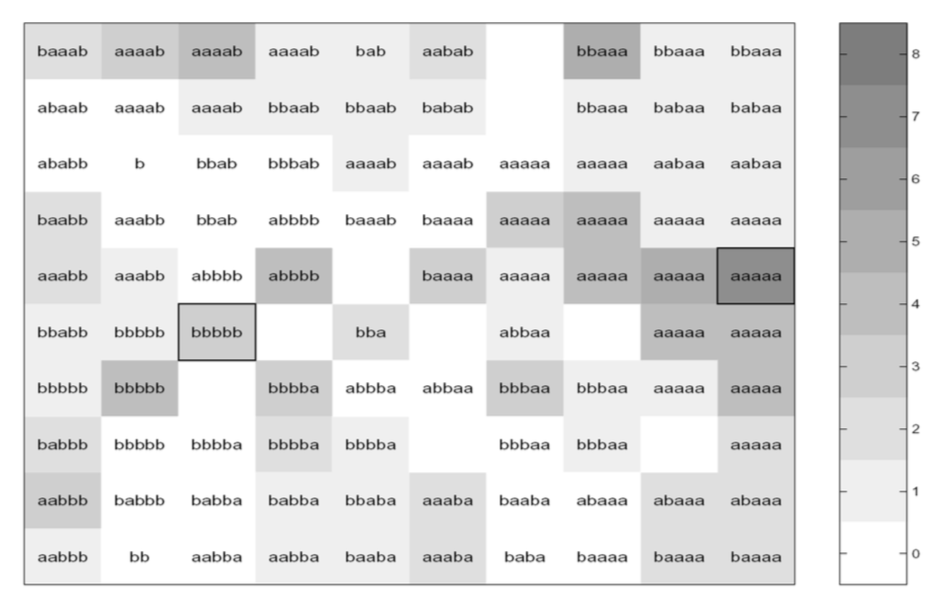
\includegraphics[width=10cm]{assets/receptive_field}
	\caption{Ukážka hitmapy}
\end{figure}

\section{Pamäťová hĺbka SRN s Elmanovou architektúrou}
SRN s Elmanovou architektúrou sme chceli porovnať s rekurentnými SOM najmä z toho dôvodu, že má niektoré vlastnosti spoločné 
so SOM. Ak by sme odstránili výstupnú vrstvu, tak dostaneme architektúru rekurentnej SOM.
Prekážkou je, že odmerať a hlavne porovnať pamäťovú hĺbku takejto siete s inými sieťami nie je jednoduché, keďže má úplne odlišnú architektúru.
Pokúšali sme sa nájsť spôsob ako odmerať pamäťovú hĺbku takejto siete.
Navrhli sme riešenie, pomocou ktorého vieme vizualizovať vzdialenosti medzi stavmi na kontextovej vrstve siete, ale
na základe týchto informácii sme nedokázali rozumne kvantifikovať pamäťovú hĺbku takejto siete a teda 
ani ju porovnať s rekurentnými SOM.


\section{Výber vhodných trénovacích dát}
Trénovacie sekvencie sú tvorené písmenami anglickej abecedy (26 písmen).
Spoločnou vlastnosťou týchto trénovacích sekvencií je, že sú tvorené/generované určitým nenáhodným spôsobom (obsahujú napríklad opakujúce sa podsekvencie)
a teda môžeme na nich trénovať rekurentné neurónové siete. 
Inými slovami dokážu v nich rekurentné neurónové siete zachytiť určité vzory a opakovania, ktoré si pamätajú vo svojom kontexte.
Samotné vstupy (trénovacie príklady) pre sieť sú kódované jednotlivé písmená \\ z trénovacej sekvencie.
Keďže neurónové siete vedia najlepšie pracovať s vektormi číselných hodnôt, jednotlivé vstupné znaky zo 
vstupnej sekvencie kódujeme počas trénovania do 26 prvkového vektora metódou one-hot, 
a teda jeho prvky sú nuly a jednotka (pre každé písmeno je jednotka na unikátnej pozícii).
Napríklad písmeno A bude reprezentované vektorom
$[1, 0, 0, 0, 0, 0, 0, 0, 0, 0, 0, 0, 0, 0, 0, 0, 0, 0, 0, 0, 0, 0, 0, 0]$,
písmeno B vektorom $[0, 1, 0, 0, 0, 0, 0, 0, 0, 0, 0, 0, 0, 0, 0, 0, 0, 0, 0, 0, 0, 0, 0, 0]$ atď. 
ktorý bude na vstupe neurónovej siete.
Tento spôsob reprezentácie vstupov pre sieť je jednoduchý a siete s ním vedia dobre pracovať.


\section {Návrh experimentu}
Experiment sme rozdelili na 2 hlavné časti. 
Prvá časť experimentu sa venuje meraniu pamäťovej hĺbky rekurentných SOM a hľadanie 
optimálnych parametrov, pri ktorých dosahujú najvyššie hodnoty pamäťových hĺbok. \\
V tejto časti sa venujeme tiež analýze výsledkov a hľadaniu súvislostí medzi veľkosťou pamäťovej hĺbky 
a hodnotami parametrov. 
Na záver sme spravili porovnanie pamäťových hĺbok všetkých testovaných typov rekurentných SOM s 
použitím optimálnych váh a fixnou inicializáciou váh.
V druhej časti experimentu sa venujeme pokusu s SRN a vizualizácii vnútorných stavov siete vo forme 
dendogramu a vyhodnoteniu výsledkov.

Experiment so rekurentnými SOM prebieha nasledujúcim spôsobom:
\begin{itemize}
    \item Výber vhodnej trénovacej sekvencie, počtu epôch trénovania a vhodnú veľkosť pamäťového okna
    \item Trénovanie siete na všetkých kombináciach týchto dvoch parametrov
    \item Ukladanie hodnot pamäťovej hĺbky a kvantizačných chýb do súboru
    \item Vykreslenie heatmapy, ktorá znázorňuje aká bola pamäťová hĺbka pre rôzne kombinácie parametrov.
    \item Testovanie pamäťovej hĺbky sietí s optimálnymi parametrami na rôznych trénovacích dátach.
    \item Vyhodnotenie a analýza výsledkov
\end{itemize}







